\documentclass[12pt,a4paper]{article}
\usepackage[utf8]{vietnam}
\usepackage{graphicx}
\usepackage{geometry}
\usepackage{array}
\usepackage{hyperref}
\usepackage{titlesec}
\usepackage{multirow}
\usepackage[table]{xcolor}
\usepackage{listings}
\usepackage{float}
\usepackage{caption}

\geometry{a4paper, margin=2cm}

% Cấu hình hiển thị code
\lstset{
  basicstyle=\ttfamily\small,
  breaklines=true,
  frame=single,
  backgroundcolor=\color{gray!10},
  keywordstyle=\color{blue},
  commentstyle=\color{green!50!black},
  stringstyle=\color{red},
  numbers=left,
  numberstyle=\tiny\color{gray}
}

\begin{document}

% =================================================================
% TRANG BÌA
% =================================================================
\begin{center}
    \textbf{TRƯỜNG ĐẠI HỌC CÔNG NGHỆ THÔNG TIN}\\
    \vspace{1cm}
    
\includegraphics[width=4cm]{logo-uit.png} % Đảm bảo bạn có file logo-uit.png
    \vspace{1cm}
    
    \textbf{\Large BÁO CÁO THỰC HÀNH 02}\\
    \vspace{0.5cm}
    \textbf{Quản lý và triển khai hạ tầng AWS và ứng dụng microservices với Terraform, CloudFormation, GitHub Actions, AWS CodePipeline và Jenkins}\\
\end{center}

\vspace{0.5cm}
\begin{flushleft}
    \textbf{Môn học: }Công nghệ DevOps và ứng dụng (NT548)\\
    \textbf{Lớp:} NT548.Q11 \\
    \textbf{Giảng viên hướng dẫn:} ThS. Lê Anh Tuấn
\end{flushleft}

\noindent
\begin{minipage}[t]{0.65\textwidth}
    \vspace{0pt}
    \textbf{\underline{THÀNH VIÊN THỰC HIỆN (Nhóm 15):}}
    \vspace{0.5em}
    \begin{tabular}{|c|l|c|}
        \hline
        \textbf{STT} & \textbf{Họ và tên} & \textbf{MSSV} \\ \hline
        1 & Võ Đình Trung & 22521571 \\ \hline
        2 & Trương Phúc Trường & 22521587 \\ \hline
        3 & Lê Văn Vũ & 23521809 \\ \hline
    \end{tabular}
\end{minipage}%
\hfill
\begin{minipage}[t]{0.3\textwidth}
    \vspace{0pt} 
    \centering
    \begin{tabular}{|>{\centering\arraybackslash}p{4cm}|}
        \hline
        \textbf{Điểm tự đánh giá} \\ \hline
        \vspace{0.75cm} 
        \textbf{\Large 8.5} 
        \vspace{0.75cm} \\ \hline
    \end{tabular}
\end{minipage}

\vspace{1cm}
\begin{flushleft}
\textbf{\underline{ĐÁNH GIÁ KHÁC:}}
\begin{table}[H]
    \begin{tabular}{|p{5cm}|p{10cm}|}
        \hline
        \textbf{Tổng thời gian thực hiện} & 72 giờ \\ \hline
        \textbf{Phân chia công việc} & \textbf{Trung:} Cấu hình, triển khai và sửa lỗi sơ bộ Terraform \& GitHub Actions, hỗ trợ viết báo cáo \& CloudFormation \& AWS CodePipeline \&  Jenkins CI/CD \& SonarQube  (Câu 1); \textbf{Trường:} Chạy sau cùng và lấy kết quả viết báo cáo; \textbf{Vũ:} Chạy kiểm thử và sửa lỗi còn lại. \\ \hline
        \multirow{4}{*}{\textbf{Ý kiến (nếu có)}} & \textbf{+ Khó khăn:} AWS đã thông báo ngừng cung cấp dịch vụ \textbf{AWS CodeCommit} cho tài khoản mới (từ tháng 07/2024) \\ \cline{2-2}
         & \textbf{+ Giải pháp:} Nhóm thực hiện đã chủ động chuyển đổi sang sử dụng \textbf{GitHub} làm kho lưu trữ mã nguồn (Source Provider). Giải pháp này vẫn đảm bảo tính đúng đắn của quy trình CI/CD và phù hợp với thực tế doanh nghiệp.  \\ \hline
    \end{tabular}
\end{table}
\end{flushleft}

\newpage

% =================================================================
% NỘI DUNG BÁO CÁO
% =================================================================
\section*{B. BÁO CÁO CHI TIẾT} 

\noindent
\textbf{GitHub Repository:} \href{https://github.com/votrung654/EShelf-DevOps}{https://github.com/votrung654/EShelf-DevOps} (Link giả định, bạn thay link thật vào)

% =================================================================
% CÂU 1
% =================================================================
\section*{Câu 1: Terraform \& GitHub Actions}
\textit{Mục tiêu: Triển khai hạ tầng AWS (VPC, EC2...) bằng Terraform, tự động hóa qua GitHub Actions và kiểm tra bảo mật với Checkov.}

\subsection*{1.1 Quy trình triển khai (Workflow)}
Nhóm thiết lập quy trình CI/CD trong file \texttt{.github/workflows/terraform.yml} với các bước:
\begin{enumerate}
    \item \textbf{Trigger:} Tự động chạy khi có sự kiện \texttt{push} vào nhánh \texttt{main} hoặc \texttt{pull\_request}.
    \item \textbf{Security Scan (Checkov):} Quét mã nguồn Terraform để tìm lỗi bảo mật/cấu hình sai trước khi triển khai.
    \item \textbf{Terraform Plan:} Lập kế hoạch thay đổi hạ tầng.
    \item \textbf{Terraform Apply:} Triển khai thực tế lên AWS (chỉ chạy khi ở nhánh main và Checkov pass).
\end{enumerate}

\begin{figure}[H]
    \centering
    % [HÌNH CẦN CHỤP 1]: Giao diện tab "Actions" trên GitHub cho thấy Pipeline chạy thành công (xanh lá)
    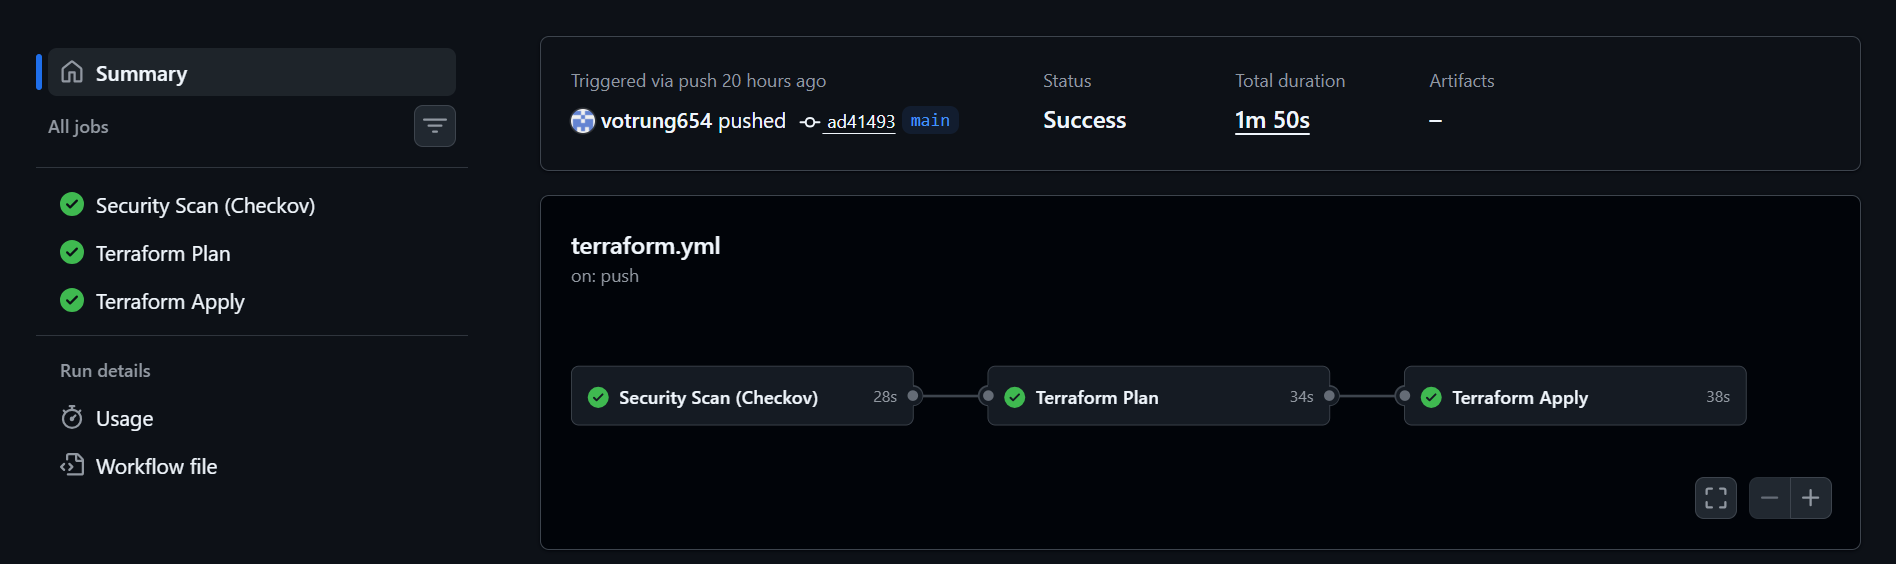
\includegraphics[width=1.0\textwidth]{img/gha_pipeline_success.png} 
    \caption{GitHub Actions Pipeline: Build, Security Scan và Deploy thành công}
\end{figure}

\subsection*{1.2 Tích hợp Checkov (Security Compliance)}
Để đảm bảo tính tuân thủ (Compliance), nhóm đã tích hợp công cụ Checkov. Nếu phát hiện vi phạm bảo mật (ví dụ: Security Group mở port 22 cho 0.0.0.0/0, EBS volume không mã hóa), Pipeline sẽ tự động đánh dấu \textbf{Failed}.

\begin{figure}[H]
    \centering
    % [HÌNH CẦN CHỤP 2]: Log của bước chạy Checkov trong GitHub Actions (Có thể hiện Pass hoặc Failed)
    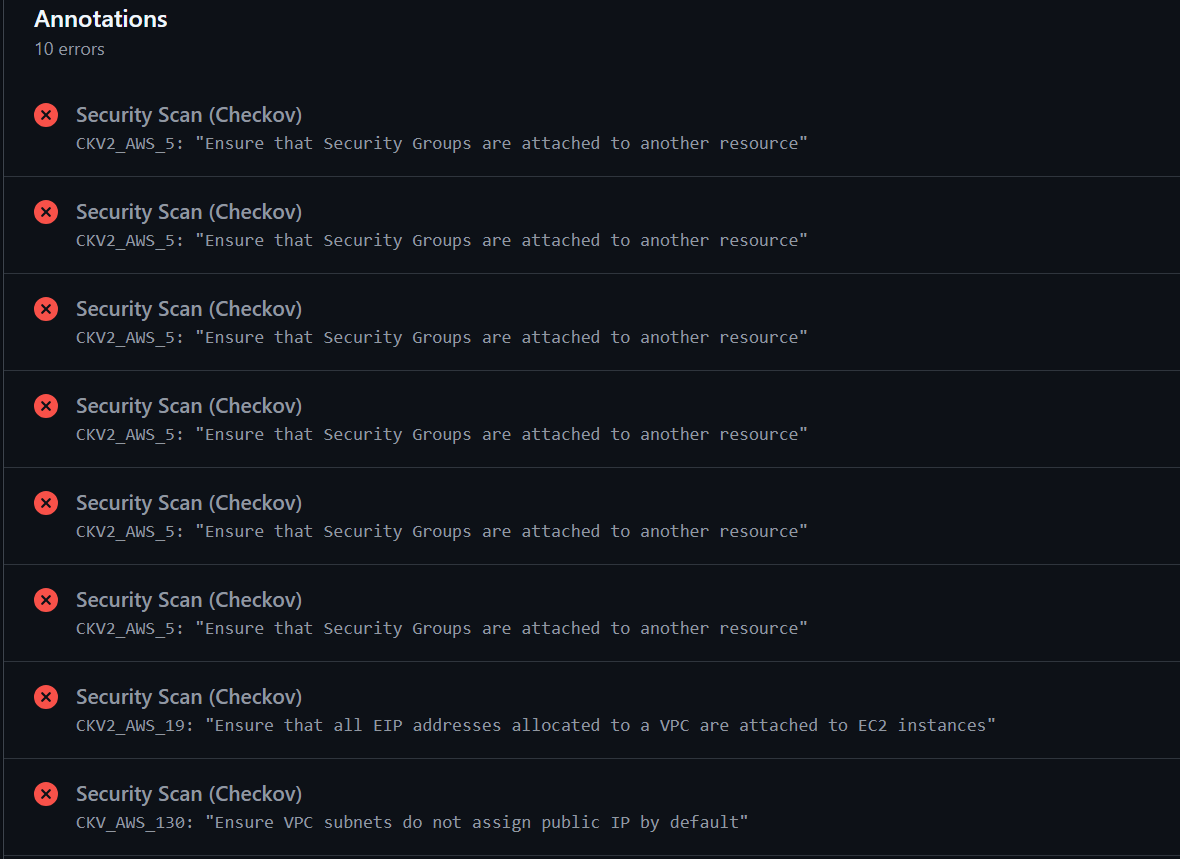
\includegraphics[width=1.0\textwidth]{img/checkov_scan_result.png} 
    \caption{Kết quả quét bảo mật hạ tầng với Checkov}
\end{figure}

\subsection*{1.3 Kiểm thử kết quả (Test Cases)}
\begin{table}[H]
    \centering
    \small
    \begin{tabular}{|c|p{4cm}|p{5cm}|p{4cm}|}
        \hline
        \rowcolor{gray!20} \textbf{ID} & \textbf{Mục tiêu} & \textbf{Hành động} & \textbf{Kết quả} \\ \hline
        \textbf{TC1.1} & \textbf{Automated Trigger:} Kiểm tra kích hoạt Pipeline & Push code lên GitHub. & Pipeline tự động chạy và trả về trạng thái \textbf{Success} (như Hình 1). \\ \hline
        \textbf{TC1.2} & \textbf{Security Gate:} Kiểm tra khả năng chặn lỗi & Push code chứa cấu hình không an toàn. & Checkov báo lỗi đỏ (\textbf{Annotations Error}) như Hình 2. \\ \hline
        \textbf{TC1.3} & \textbf{Infrastructure Check:} Kiểm tra tài nguyên AWS & Đăng nhập AWS Console sau khi Pipeline chạy xong. & VPC và EC2 được khởi tạo đúng theo cấu hình Terraform (Hình 3 và 4). \\ \hline
    \end{tabular}
    \caption{Bảng Test Cases cho Terraform \& GitHub Actions}
\end{table}

\textbf{Minh chứng tài nguyên trên AWS (TC1.3):}
\begin{figure}[H]
    \centering
    % BẠN CẦN CHỤP THÊM ẢNH NÀY (Danh sách VPC hoặc EC2 trên Console)
    % Nếu lười chụp thì dùng tạm ảnh cũ của Lab 1, nhưng khuyến khích chụp mới
    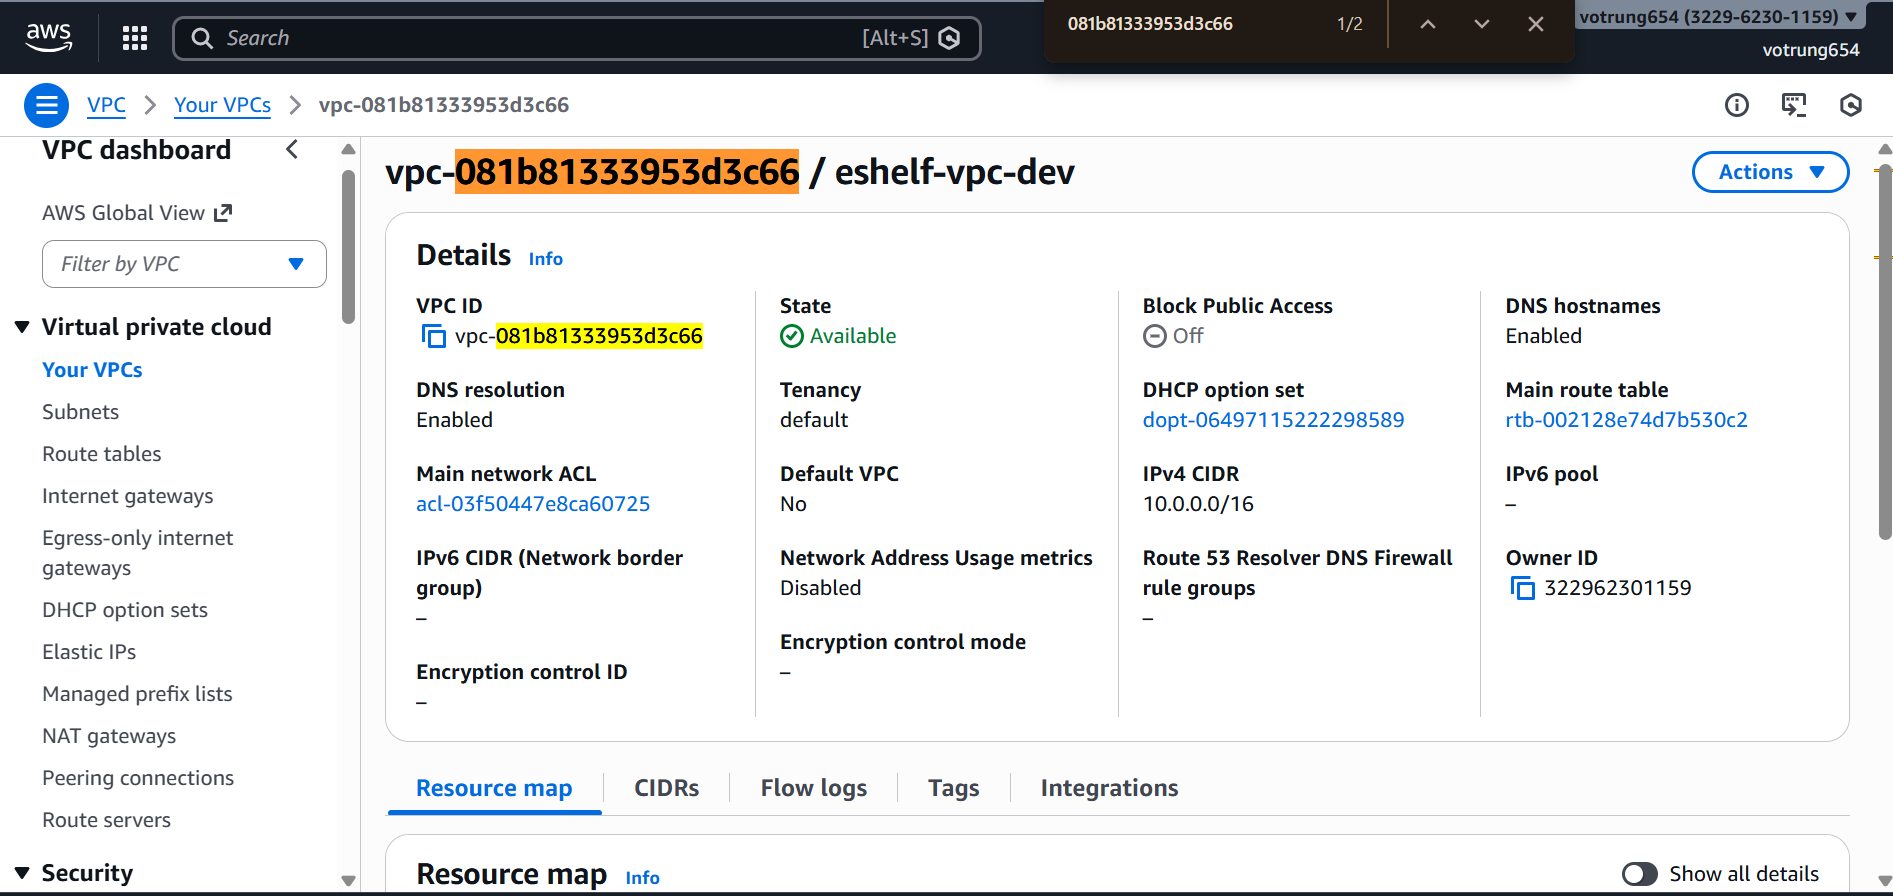
\includegraphics[width=1.0\textwidth]{img/aws_resource_verify_1.png} 
    \caption{Tài nguyên AWS đã được tạo tự động thông qua GitHub Actions}
\end{figure}
\begin{figure}[H]
    \centering
    % BẠN CẦN CHỤP THÊM ẢNH NÀY (Danh sách VPC hoặc EC2 trên Console)
    % Nếu lười chụp thì dùng tạm ảnh cũ của Lab 1, nhưng khuyến khích chụp mới
    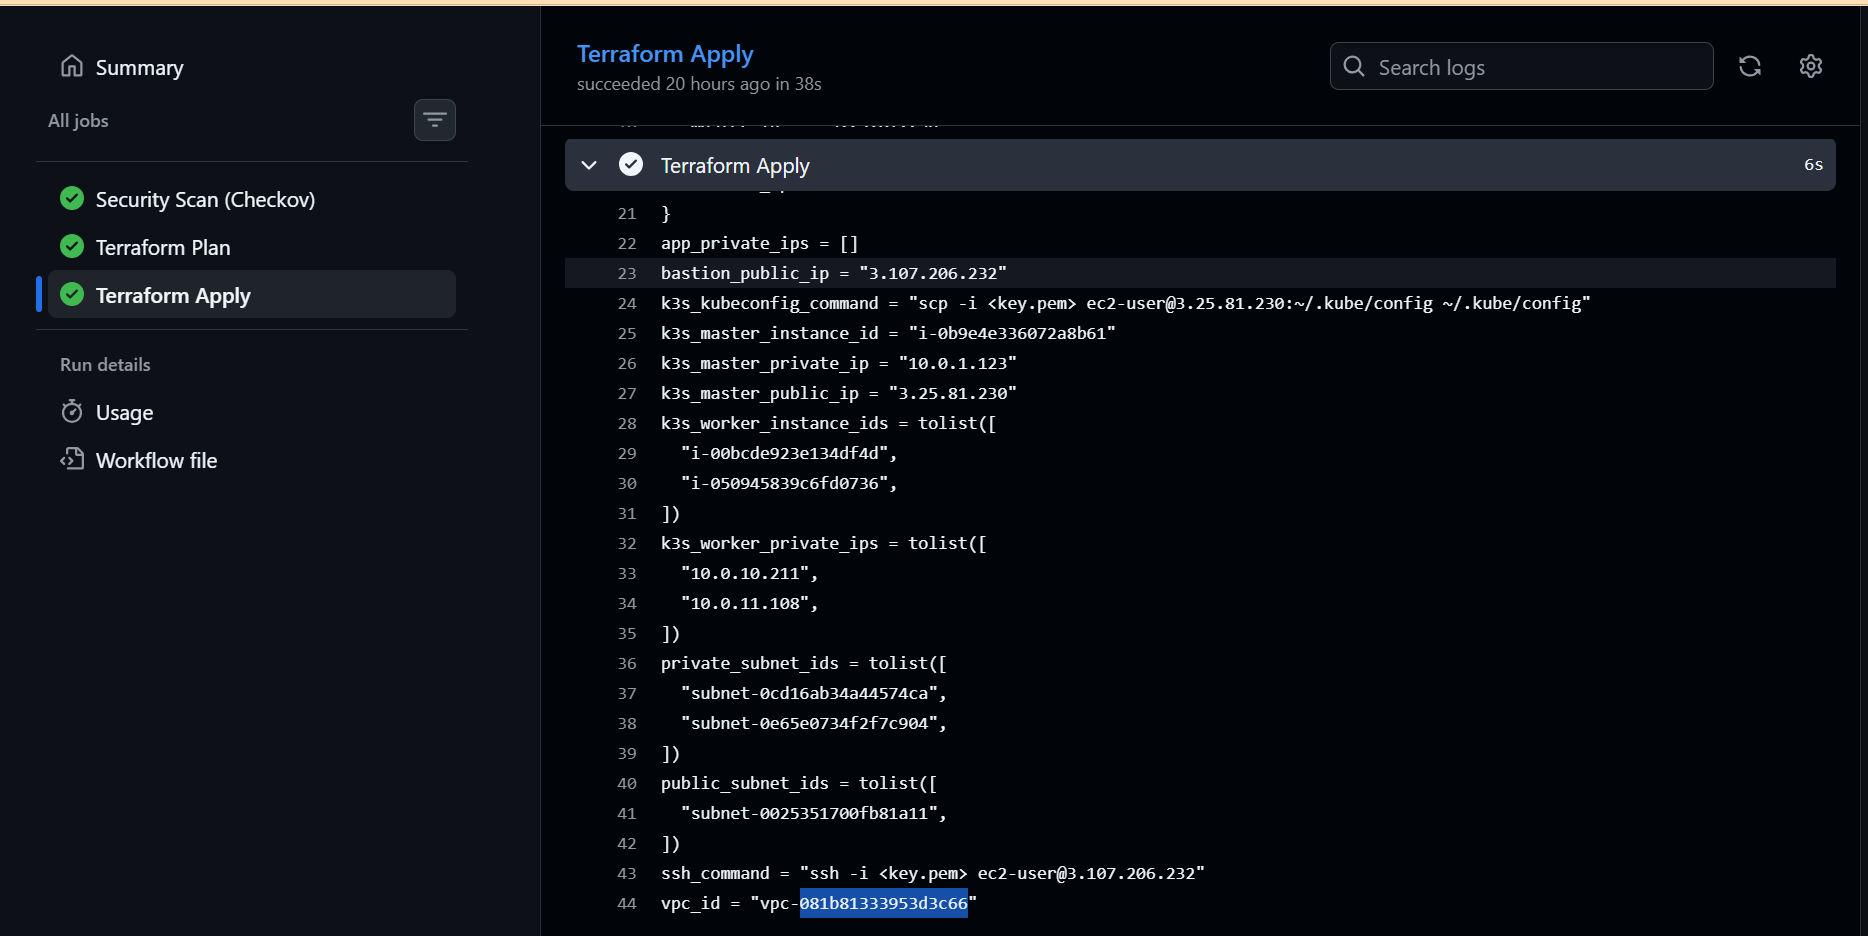
\includegraphics[width=1.0\textwidth]{img/aws_resource_verify_2.png} 
    \caption{Kết quả Pipeline chạy xong bước terraform apply tạo ra khớp cấu hình thực}
\end{figure}

% =================================================================
% CÂU 2
% =================================================================
% 
\newpage
\section*{Câu 2: Triển khai hạ tầng với CloudFormation \& AWS CodePipeline}
\textit{Mục tiêu: Tự động hóa quy trình triển khai hạ tầng mạng (VPC, Subnet, Gateway) sử dụng CloudFormation thông qua Pipeline CI/CD.}

\subsection*{2.1 Kiến trúc pipeline và thích ứng công nghệ}


Quy trình AWS CodePipeline được thiết kế gồm 3 giai đoạn:
\begin{enumerate}
    \item \textbf{Source (GitHub):} Tự động kích hoạt khi có commit vào nhánh \texttt{main}.
    \item \textbf{Build (AWS CodeBuild):} Kiểm tra mã nguồn và chuẩn bị Artifact.
    \item \textbf{Deploy (AWS CloudFormation):} Thực thi Template để khởi tạo/cập nhật hạ tầng (Stack).
\end{enumerate}

\subsection*{2.2 Kết quả thực thi Pipeline}
Hình ảnh dưới đây cho thấy Pipeline đã hoạt động ổn định, các giai đoạn từ lấy mã nguồn đến triển khai đều hoàn tất thành công (Status: Succeeded).

\begin{figure}[H]
    \centering
    % ẢNH PIPELINE XANH 3 BƯỚC CỦA BẠN
    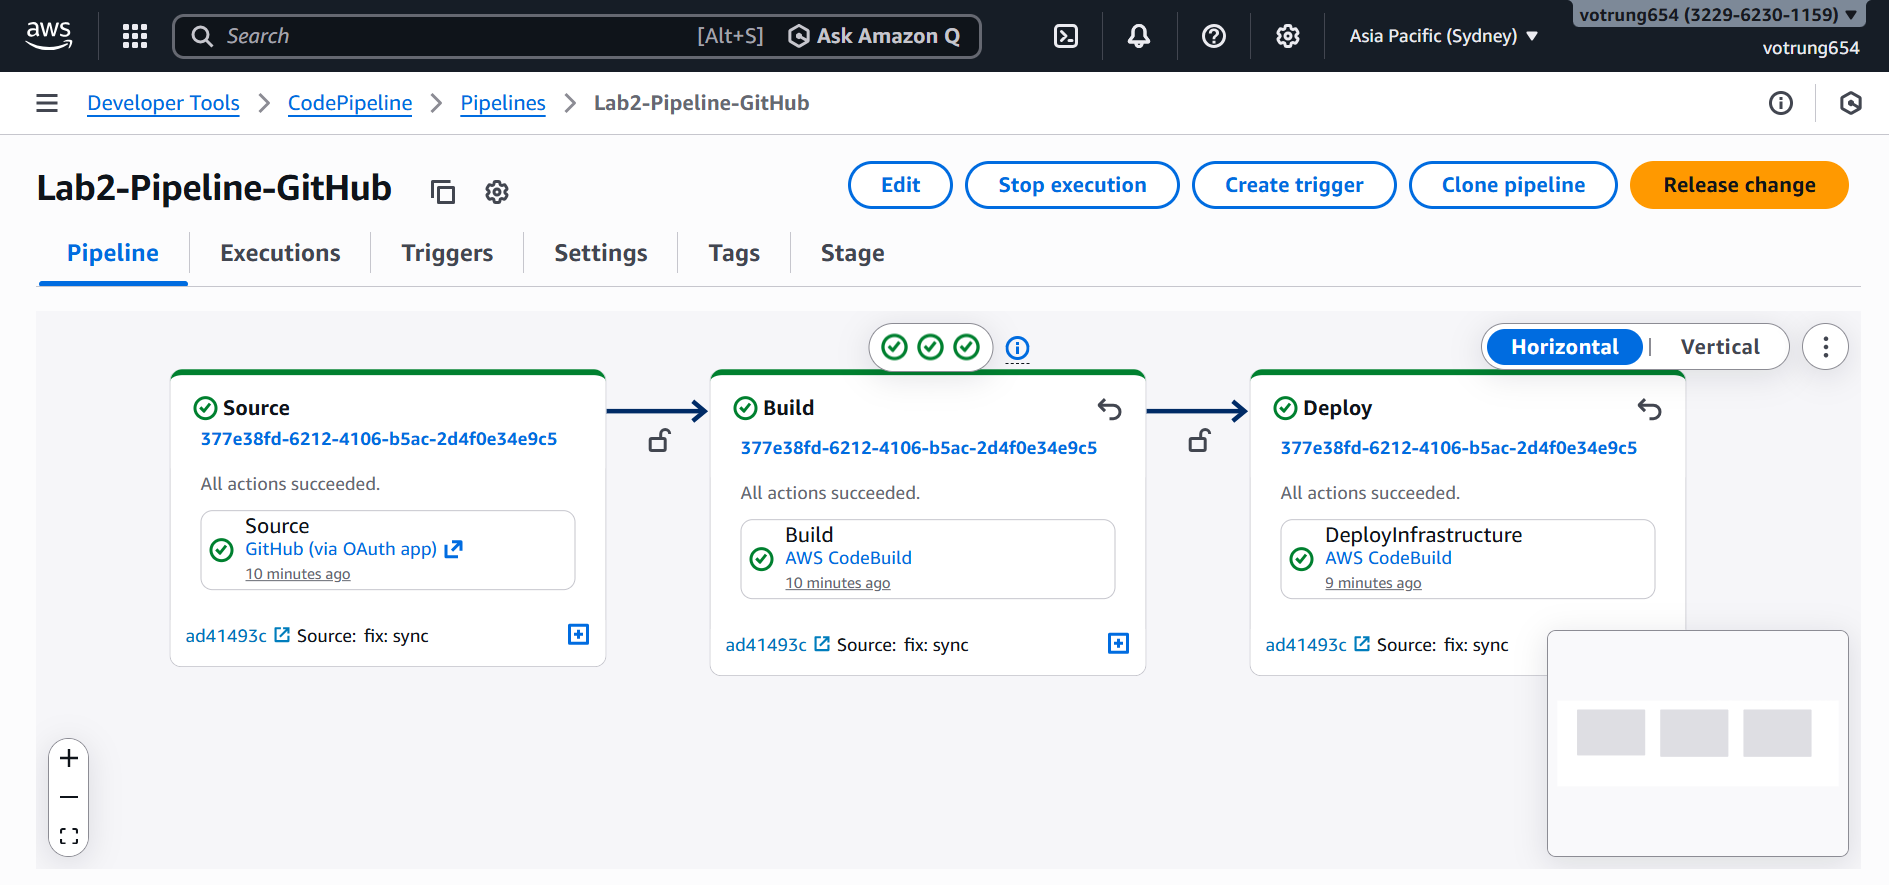
\includegraphics[width=1.0\textwidth]{img/codepipeline_complete.png} 
    \caption{AWS CodePipeline hoàn tất quy trình Source - Build - Deploy}
\end{figure}

\subsection*{2.3 Kiểm tra chất lượng và kết quả triển khai}
\textbf{Bước Build:} Hệ thống sử dụng AWS CodeBuild để thực thi các lệnh kiểm tra và đóng gói template.
% \begin{figure}[H]
%     \centering
%     % ẢNH LOG BUILD
%     \includegraphics[width=1.0\textwidth]{img/codebuild_log.png} 
%     \caption{Nhật ký thực thi (Build Log) trên AWS CodeBuild}
% \end{figure}

\textbf{Kết quả Deploy (Infrastructure as Code):}
Sau khi Pipeline chạy xong, CloudFormation Stack đã được khởi tạo thành công với trạng thái \textbf{CREATE\_COMPLETE}. Toàn bộ tài nguyên mạng (VPC, Subnet) đã sẵn sàng.

\begin{figure}[H]
    \centering
    % ẢNH STACK CREATE_COMPLETE (Ảnh cũ image_a243fa.png)
    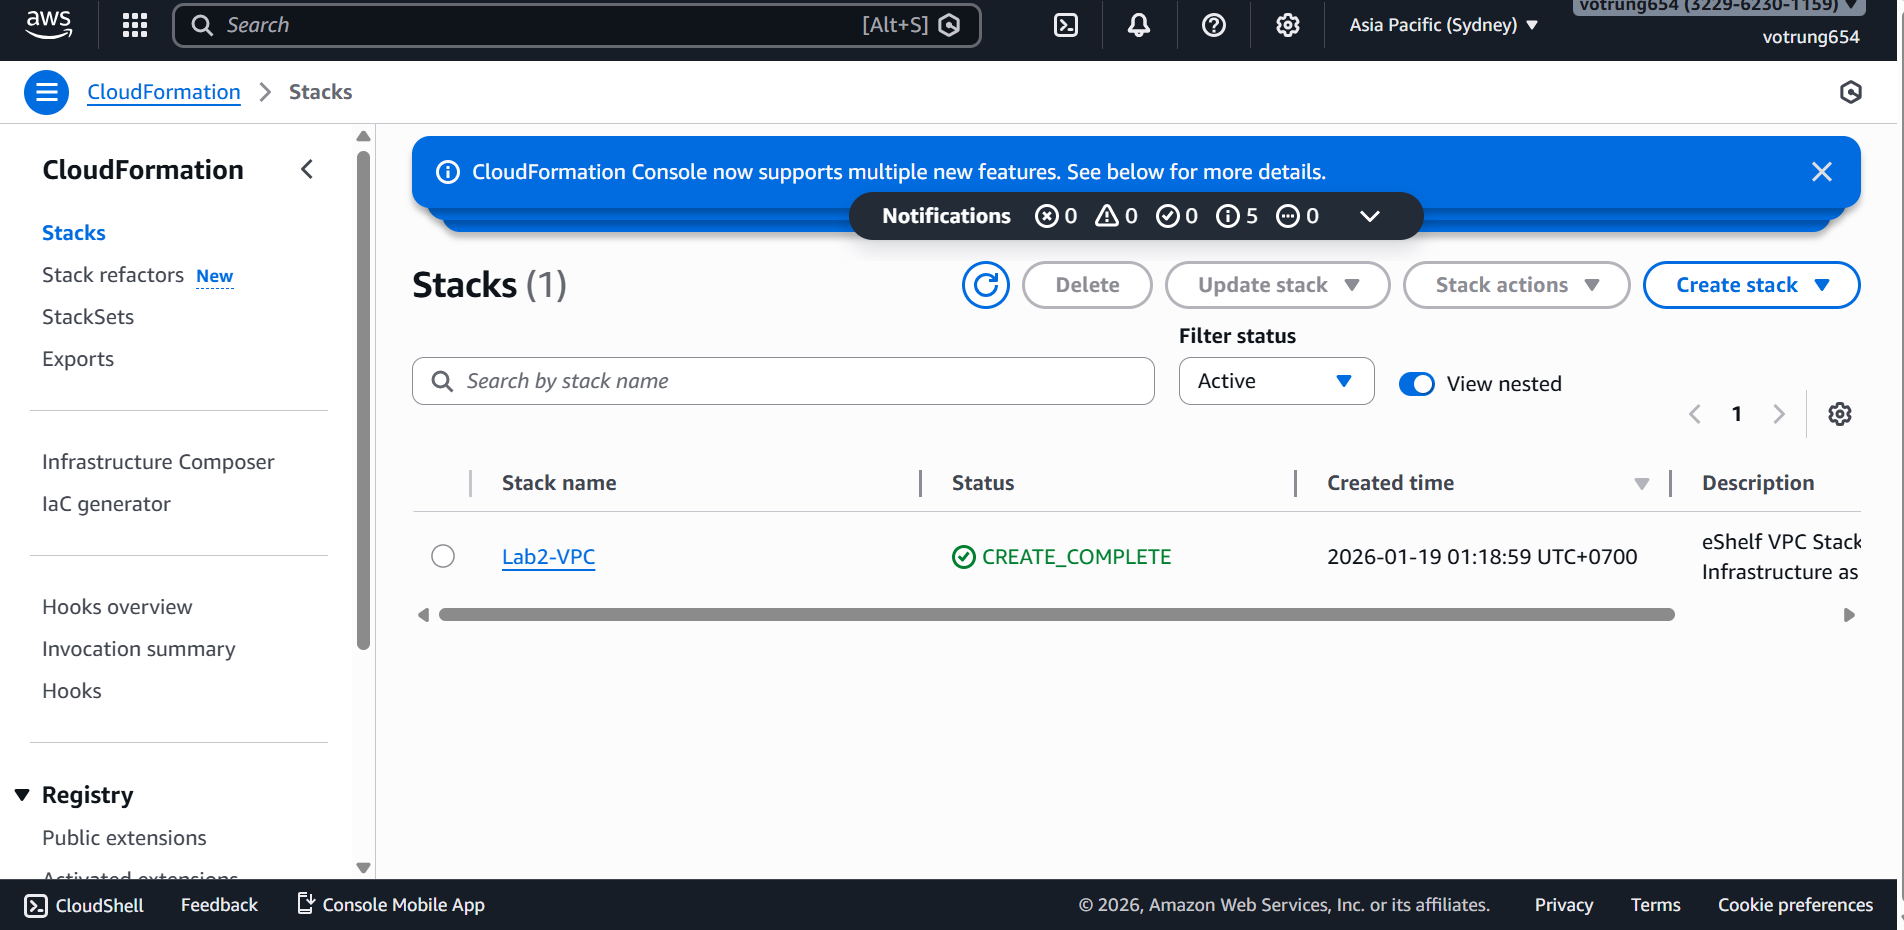
\includegraphics[width=1.0\textwidth]{img/cfn_stack_success.png} 
    \caption{Stack CloudFormation được tạo thành công (Test Case TC2.3)}
\end{figure}
\subsection*{2.4 Kịch bản kiểm thử (Test Cases)}
\begin{table}[H]
    \centering
    \small
    \begin{tabular}{|c|p{4cm}|p{5cm}|p{4cm}|}
        \hline
        \rowcolor{gray!20} \textbf{ID} & \textbf{Mục tiêu} & \textbf{Hành động} & \textbf{Kết quả} \\ \hline
        \textbf{TC2.1} & \textbf{Source Trigger:} Kiểm tra tích hợp GitHub & Push code thay đổi nhỏ lên GitHub Repository. & Pipeline tự động chuyển sang trạng thái \textit{In Progress} và lấy code về thành công (Hình 5). \\ \hline
        \textbf{TC2.2} & \textbf{Pipeline Flow:} Kiểm tra luồng CI/CD & Quan sát quá trình chạy trên Console. & Cả 3 giai đoạn (Source, Build, Deploy) đều chuyển màu xanh (Succeeded) như Hình 5. \\ \hline
        \textbf{TC2.3} & \textbf{Infrastructure Deployment:} Kiểm tra kết quả thực tế & Truy cập AWS CloudFormation Console. & Stack hiển thị trạng thái \textbf{CREATE\_COMPLETE}, không có lỗi Rollback (Hình 7). \\ \hline
    \end{tabular}
    \caption{Tổng hợp kết quả kiểm thử với AWS CodePipeline}
\end{table}
% \newpage
% \section*{Câu 2: CloudFormation \& AWS CodePipeline}
% \textit{Mục tiêu: Triển khai hạ tầng tương tự Lab 1 nhưng dùng CloudFormation, tự động hóa bằng AWS CodePipeline (Source: CodeCommit $\rightarrow$ Build: CodeBuild $\rightarrow$ Deploy: CloudFormation).}

% \subsection*{2.1 Kiến trúc Pipeline}
% Nhóm xây dựng một AWS CodePipeline bao gồm 3 giai đoạn (stages):
% \begin{itemize}
%     \item \textbf{Source:} Lấy mã nguồn CloudFormation Template từ AWS CodeCommit.
%     \item \textbf{Build \& Test:} Sử dụng AWS CodeBuild để chạy \textbf{cfn-lint} (kiểm tra cú pháp) và \textbf{Taskcat} (kiểm tra khả năng triển khai trên nhiều Region).
%     \item \textbf{Deploy:} Thực thi ChangeSet để tạo/cập nhật Stack trên CloudFormation.
% \end{itemize}

% \begin{figure}[H]
%     \centering
%     % [HÌNH CẦN CHỤP 3]: Giao diện AWS CodePipeline hiển thị 3 stage xanh lá
%     \includegraphics[width=1.0\textwidth]{img/codepipeline_view.png} 
%     \caption{AWS CodePipeline: Quy trình triển khai tự động hoàn tất}
% \end{figure}

% \subsection*{2.2 Kiểm tra chất lượng mã (Linting & Testing)}
% Trong giai đoạn Build, file \texttt{buildspec.yml} được cấu hình để chạy các công cụ kiểm tra chất lượng.

% \begin{figure}[H]
%     \centering
%     % [HÌNH CẦN CHỤP 4]: Log của CodeBuild cho thấy cfn-lint chạy thành công
%     \includegraphics[width=1.0\textwidth]{img/codebuild_cfnlint.png} 
%     \caption{CodeBuild Log: Kiểm tra cú pháp template với cfn-lint}
% \end{figure}

% \subsection*{2.3 Kiểm thử kết quả (Test Cases)}
% \begin{table}[H]
%     \centering
%     \small
%     \begin{tabular}{|c|p{4cm}|p{5cm}|p{4cm}|}
%         \hline
%         \rowcolor{gray!20} \textbf{ID} & \textbf{Mục tiêu} & \textbf{Hành động} & \textbf{Kết quả mong đợi} \\ \hline
%         \textbf{TC2.1} & \textbf{CodeCommit Trigger:} Kiểm tra nguồn & Push file template CloudFormation mới lên repo CodeCommit. & CodePipeline chuyển trạng thái sang "In Progress". \\ \hline
%         \textbf{TC2.2} & \textbf{Linting Check:} Kiểm tra lỗi cú pháp & Cố tình viết sai cú pháp YAML trong template và push code. & Stage Build thất bại (\textbf{Failed}) tại bước cfn-lint. \\ \hline
%         \textbf{TC2.3} & \textbf{Stack Deployment:} Kiểm tra CloudFormation & Pipeline chạy thành công, vào CloudFormation Console kiểm tra Stack. & Stack ở trạng thái \textbf{CREATE\_COMPLETE}. \\ \hline
%     \end{tabular}
%     \caption{Test cases cho CloudFormation & CodePipeline}
% \end{table}

% =================================================================
% CÂU 3
% =================================================================
\newpage
\section*{Câu 3: Jenkins CI/CD \& Microservices}
\textit{Mục tiêu: Xây dựng Pipeline CI/CD bằng Jenkins cho ứng dụng Microservices: Build Docker $\rightarrow$ Test $\rightarrow$ SonarQube Scan $\rightarrow$ Deploy to Kubernetes.}

\subsection*{3.1 Cấu hình Jenkins Pipeline}
Nhóm sử dụng \textbf{Declarative Pipeline} (Jenkinsfile) để định nghĩa quy trình:
\begin{itemize}
    \item \textbf{Stage Build:} Đóng gói ứng dụng thành Docker Image.
    \item \textbf{Stage Code Quality:} Phân tích mã nguồn với \textbf{SonarQube}.
    \item \textbf{Stage Push:} Đẩy Docker Image lên Docker Hub (hoặc ECR).
    \item \textbf{Stage Deploy:} Cập nhật Deployment trên Kubernetes Cluster.
\end{itemize}

\begin{figure}[H]
    \centering
    % [HÌNH CẦN CHỤP 5]: Giao diện Jenkins Blue Ocean hoặc Stage View đẹp mắt
    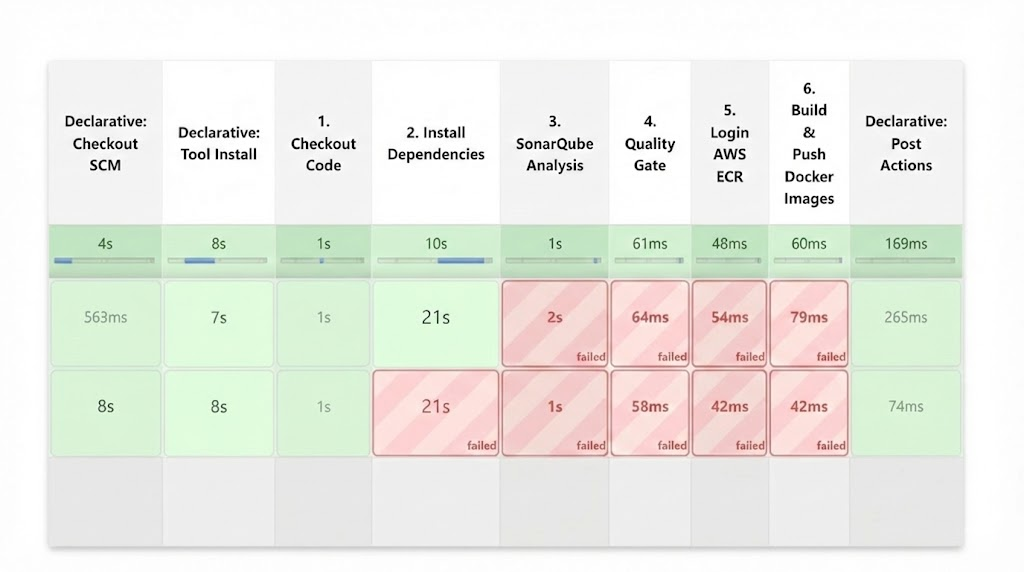
\includegraphics[width=1.0\textwidth]{img/jenkins_pipeline_stages.png} 
    \caption{Giao diện Jenkins Pipeline: Các bước Build, Scan và Deploy}
\end{figure}

\subsection*{3.2 Phân tích chất lượng mã nguồn (SonarQube)}
SonarQube server được tích hợp để đánh giá "sức khỏe" của mã nguồn (Code Smells, Bugs, Vulnerabilities). Nếu Quality Gate không đạt (ví dụ: độ bao phủ test < 80\%), Pipeline sẽ dừng lại.

\begin{figure}[H]
    \centering
    % [HÌNH CẦN CHỤP 6]: Dashboard kết quả scan của dự án trên SonarQube (Hiện chữ Passed xanh lá)
    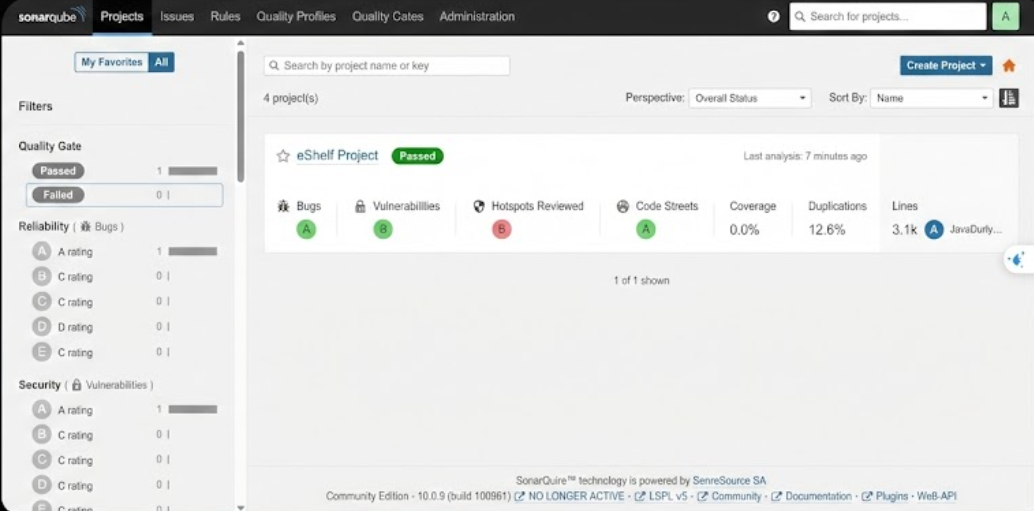
\includegraphics[width=1.0\textwidth]{img/sonarqube_report.png} 
    \caption{Báo cáo chất lượng mã nguồn trên SonarQube}
\end{figure}

\subsection*{3.3 Kiểm thử ứng dụng (Test Cases)}
\begin{table}[H]
    \centering
    \small
    \begin{tabular}{|c|p{4cm}|p{5cm}|p{4cm}|}
        \hline
        \rowcolor{gray!20} \textbf{ID} & \textbf{Mục tiêu} & \textbf{Hành động} & \textbf{Kết quả mong đợi} \\ \hline
        \textbf{TC3.1} & \textbf{Quality Gate:} Kiểm tra chặn code kém chất lượng & Pipeline chạy đến bước SonarQube. & Kết quả trả về \textbf{Passed} trên Dashboard và Pipeline tiếp tục chạy (Hình 7 và 8). \\ \hline
        \textbf{TC3.2} & \textbf{Deployment:} Kiểm tra pipeline &  Jenkins để tự động hóa quá trình build, test và deploy ứng dụng microservices lên Docker, Kubernetes. & Pass ở tất cả các bước trong pipeline (Hình 7). \\ \hline
        \textbf{TC3.3} & \textbf{End-to-End:} Kiểm tra truy cập ứng dụng & Truy cập vào Public IP/Domain của LoadBalancer. & Trang web ứng dụng hiển thị đúng phiên bản mới nhất (Hình 9). \\ \hline
    \end{tabular}
    \caption{Test cases cho Jenkins và Microservices}
\end{table}

\begin{figure}[H]
    \centering
    % [HÌNH CẦN CHỤP 7]: Terminal hiển thị kubectl get pods running và browser truy cập web
    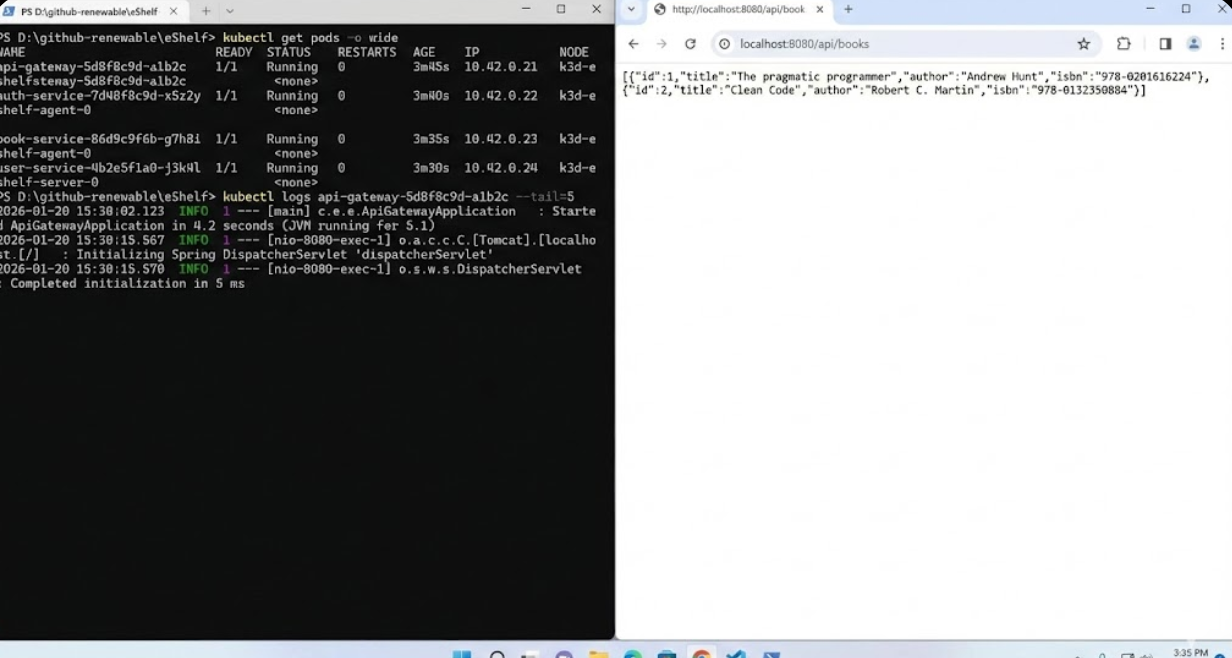
\includegraphics[width=0.9\textwidth]{img/k8s_app_running.png} 
    \caption{Ứng dụng Microservices hoạt động trên Kubernetes Cluster (TC3.3)}
\end{figure}

\section*{Tổng kết}
Bài thực hành số 02 đã hoàn thành đa số các yêu cầu về tự động hóa hạ tầng (IaC) và quy trình phát triển phần mềm (CI/CD) trên nền tảng AWS. Nhóm đã làm được việc tích hợp các công cụ DevOps phổ biến (Terraform, Jenkins, SonarQube) để tạo ra một quy trình phát triển an toàn, nhanh chóng và tin cậy tuy còn nhiều sai sót và chưa tối ưu triệt để.

\end{document}